% Impala Operating System
%
% Copyright (C) 2009 University of Wroclaw. Department of Computer Science
%    http://www.ii.uni.wroc.pl/
% Copyright (C) 2009 Mateusz Kocielski, Artur Koninski, Pawel Wieczorek
%    http://trzask.codepainters.com/impala/trac/
% All rights reserved.
%
% Redistribution and use in source and binary forms, with or without
% modification, are permitted provided that the following conditions
% are met:
% 1. Redistributions of source code must retain the above copyright
%  notice, this list of conditions and the following disclaimer.
% 2. Redistributions in binary form must reproduce the above copyright
%  notice, this list of conditions and the following disclaimer in the
%  documentation and/or other materials provided with the distribution.
%
% THIS SOFTWARE IS PROVIDED BY AUTHOR AND CONTRIBUTORS ``AS IS'' AND
% ANY EXPRESS OR IMPLIED WARRANTIES, INCLUDING, BUT NOT LIMITED TO, THE
% IMPLIED WARRANTIES OF MERCHANTABILITY AND FITNESS FOR A PARTICULAR PURPOSE
% ARE DISCLAIMED.  IN NO EVENT SHALL AUTHOR OR CONTRIBUTORS BE LIABLE
% FOR ANY DIRECT, INDIRECT, INCIDENTAL, SPECIAL, EXEMPLARY, OR CONSEQUENTIAL
% DAMAGES (INCLUDING, BUT NOT LIMITED TO, PROCUREMENT OF SUBSTITUTE GOODS
% OR SERVICES; LOSS OF USE, DATA, OR PROFITS; OR BUSINESS INTERRUPTION)
% HOWEVER CAUSED AND ON ANY THEORY OF LIABILITY, WHETHER IN CONTRACT, STRICT
% LIABILITY, OR TORT (INCLUDING NEGLIGENCE OR OTHERWISE) ARISING IN ANY WAY
% OUT OF THE USE OF THIS SOFTWARE, EVEN IF ADVISED OF THE POSSIBILITY OF
% SUCH DAMAGE.
%
% $Id$

\chapter{Dokumentacja techniczna.}

Nieniejszy rozdzia� opisuje techniczne aspekty naszego systemu operacyjnego.
W~tym rozdziale m�wi�c system, b�dziemy mieli na~my�li jedynie kod j�dra
systemu operacyjnego, a m�wi�c u�ytkownik b�dziemy mieli na~my�li jedynie
kod program�w dzia�aj�cych pod kontrol� naszego systemu.
S�owa klient b�dziemy u�ywaj�� w~stosunku do mechanizmu lub
procedury w~systemie wykorzystuj�c� inny mechanizm, np klientem procedury
\texttt{str\_len} jest ka�da procedura, kt�ra z niej korzysta. Klienetem
mechanizmu buforowanego wej�cia-wyj�cia jest implementacja systemu plik�w
FAT12.

% Impala Operating System
%
% Copyright (C) 2009 University of Wroclaw. Department of Computer Science
%    http://www.ii.uni.wroc.pl/
% Copyright (C) 2009 Mateusz Kocielski, Artur Koninski, Pawel Wieczorek
%    http://trzask.codepainters.com/impala/trac/
% All rights reserved.
%
% Redistribution and use in source and binary forms, with or without
% modification, are permitted provided that the following conditions
% are met:
% 1. Redistributions of source code must retain the above copyright
%  notice, this list of conditions and the following disclaimer.
% 2. Redistributions in binary form must reproduce the above copyright
%  notice, this list of conditions and the following disclaimer in the
%  documentation and/or other materials provided with the distribution.
%
% THIS SOFTWARE IS PROVIDED BY AUTHOR AND CONTRIBUTORS ``AS IS'' AND
% ANY EXPRESS OR IMPLIED WARRANTIES, INCLUDING, BUT NOT LIMITED TO, THE
% IMPLIED WARRANTIES OF MERCHANTABILITY AND FITNESS FOR A PARTICULAR PURPOSE
% ARE DISCLAIMED.  IN NO EVENT SHALL AUTHOR OR CONTRIBUTORS BE LIABLE
% FOR ANY DIRECT, INDIRECT, INCIDENTAL, SPECIAL, EXEMPLARY, OR CONSEQUENTIAL
% DAMAGES (INCLUDING, BUT NOT LIMITED TO, PROCUREMENT OF SUBSTITUTE GOODS
% OR SERVICES; LOSS OF USE, DATA, OR PROFITS; OR BUSINESS INTERRUPTION)
% HOWEVER CAUSED AND ON ANY THEORY OF LIABILITY, WHETHER IN CONTRACT, STRICT
% LIABILITY, OR TORT (INCLUDING NEGLIGENCE OR OTHERWISE) ARISING IN ANY WAY
% OUT OF THE USE OF THIS SOFTWARE, EVEN IF ADVISED OF THE POSSIBILITY OF
% SUCH DAMAGE.
%
% $Id$


\section{Zarz�dzanie pami�ci�}



% Impala Operating System
%
% Copyright (C) 2009 University of Wroclaw. Department of Computer Science
%    http://www.ii.uni.wroc.pl/
% Copyright (C) 2009 Mateusz Kocielski, Artur Koninski, Pawel Wieczorek
%    http://trzask.codepainters.com/impala/trac/
% All rights reserved.
%
% Redistribution and use in source and binary forms, with or without
% modification, are permitted provided that the following conditions
% are met:
% 1. Redistributions of source code must retain the above copyright
%  notice, this list of conditions and the following disclaimer.
% 2. Redistributions in binary form must reproduce the above copyright
%  notice, this list of conditions and the following disclaimer in the
%  documentation and/or other materials provided with the distribution.
%
% THIS SOFTWARE IS PROVIDED BY AUTHOR AND CONTRIBUTORS ``AS IS'' AND
% ANY EXPRESS OR IMPLIED WARRANTIES, INCLUDING, BUT NOT LIMITED TO, THE
% IMPLIED WARRANTIES OF MERCHANTABILITY AND FITNESS FOR A PARTICULAR PURPOSE
% ARE DISCLAIMED.  IN NO EVENT SHALL AUTHOR OR CONTRIBUTORS BE LIABLE
% FOR ANY DIRECT, INDIRECT, INCIDENTAL, SPECIAL, EXEMPLARY, OR CONSEQUENTIAL
% DAMAGES (INCLUDING, BUT NOT LIMITED TO, PROCUREMENT OF SUBSTITUTE GOODS
% OR SERVICES; LOSS OF USE, DATA, OR PROFITS; OR BUSINESS INTERRUPTION)
% HOWEVER CAUSED AND ON ANY THEORY OF LIABILITY, WHETHER IN CONTRACT, STRICT
% LIABILITY, OR TORT (INCLUDING NEGLIGENCE OR OTHERWISE) ARISING IN ANY WAY
% OUT OF THE USE OF THIS SOFTWARE, EVEN IF ADVISED OF THE POSSIBILITY OF
% SUCH DAMAGE.
%
% $Id$

\section{Sterowniki.}
\label{DEV}

Sterowniki urz�dze� w~systemach UNIXowych s� widoczne jako pliki. W naszym
systemie zarz�dzaniem takimi plikami zajmuje si� specjalny system plik�w
\texttt{devfs}, zamontowany w~katalogu \texttt{/dev}. Sterowniki urz�dze�
dziel� si� na~trzy kategorie:

\begin{itemize}
 \item urz�dzenia blokowe - sterowniki obs�uguj�ce takie
urz�dzenia jak
stacje dyskietek, dyski twarde itp.
 \item urz�dzenia znakowe - sterowniki obs�uguj�ce
urz�dzenie, widziane jako strumie� bajt�w.
 \item terminale - specjalny rodzaj urz�dze� znakowych.
\end{itemize}

Ka�dy sterownik dostarcza systemowi tak zwan� desk� rozdzielcz�
(\texttt{devsw\_t} - \emph{device switch}), kt�ra zawiera implementacj�
procedur obs�ugi pliku urz�dzenia. Deska rozdz. zawiera nast�puj�ce pola:
\begin{itemize}
 \item \texttt{d\_open} -
obs�uga otwarcie pliku urz�dzenia.

 \item \texttt{d\_close} -
obs�uga zamkni�cia pliku urz�dzenia.

 \item \texttt{d\_ioctl} -
bs�uga polece� kontrolnych dla~sterownika.

 \item \texttt{d\_write} -
obs�uga zlecenia wyj�cie ze strumienia znakowego. mo�e blokowa� klienta
na~czas wykonywania operacji.

 \item \texttt{d\_read} -
obs�uga zlecenia wej�cie ze strumienia znakowego, mo�e blokowa� klienta
na~czas wykonywania operacji.

 \item \texttt{d\_strategy} -
obs�uga zlece� operacji wej�cia-wyj�cia na~urz�dzeniach blokowych, dzia�a
asynchronicznie, tzn nie blokuje klienta na~czas wykonywania operacji.

 \item \texttt{type} -
informacja o kategorii, do jakiej urz�dzenie nale�y
\begin{itemize}
 \item \texttt{DEV\_BDEV} - dla urz�dze� blokowych.
 \item \texttt{DEV\_CDEV} - dla urz�dze� znakowych.
 \item \texttt{DEV\_TTY} - dla terminali.
\end{itemize}
\end{itemize}

Podzia� na urz�dzenia znakowego i~blokowe oraz rozr�nienie procedur
obsluguj�cych zlecenia wej�cia-wyj�cia jest koniecznie ze wzgl�du na~wydajno��
oraz obs�ug� tych urz�dze�. Na~urz�dzeniach znakowych u�ytkownik mo�e
wykonywa� te same operacje jak na plikach, poniewa� pliki s� r�wnie� widziane
jako strumienie znakowe. Dozwolone s� takie operacje jak przeczytanie jednego
bajtu, dw�ch kilobajt�w czy pi�ciu megabajt�w.

Urz�dzenia blokowe jak dyski twarde cechuje inna metod� dost�pu, fizycznie
s� one podzielone na bloki danych (sektory). St�d wszelkie transfery danych
mi�dzy pami�ci� RAM a~urz�dzeniem nie s� tak elastyczne pod~wzgl�dem wielko�ci
jak strumienie znak�w.

Z~powodu tych r�zni� jednolita obs�uga wej�cia-wyj�cia dla~tych dw�ch rodzaj�w
urz�dze� musia�aby emulowa� urz�dzenia blokowe jako znakowe, co nie by�oby
wydajne. Dzi�ki wyodr�bnienie oddzielnej procedury sterownik zawsze dostaje
zlecenia, kt�rych d�ugo�� jest wielokrotno�ci� d�ugo�ci sektoru oraz mo�e sam
zadecydowa� w~jakiej kolejno�ci najlepiej je wykona� (co t�umaczy nazw�
procedury - \emph{strategia}). Mo�liwy jest r�wnie� dost�p strumieniowy
do~takich
urz�dze�, jest on emulowany za~pomoc� procedury \texttt{physio}, kt�ra
wykorzystuje \texttt{d\_strategy}. Nale�y zwr�ci� uwag�, �e jest to~jedynie
dodatkowa metoda dost�pu, przydatna zwykle programom chc�cym bezpo�rednio
modyfikowa� dane na~urz�dzeniu lub ingerowa� w~zapisany tam system plik�w
(jak np programy sorawdzaj�ce powierzchni� dysku czy sp�jno�c systemu plik�w).
Zagadnienie wej�cja-wyj�cia urz�dze� blokowych s� om�wione w~rozdziale
\ref{BIO}.

Operacje wej�cia-wyj�cia na~terminalach dzia�aj� na~tej samej zasadzie
co urz�dze� blokowych, z~t� r�ni� �e te~operacje przechodz� dodatkow�
warstw� zwan� re�imem linii. Te zagadnienia s� szerzej om�wione w~rozdziale
TTY.

W kodzie systemu wi�kszo��, poza specjalnymi, sterownik�w jest wydzielona
do~oddzielnej biblioteki \texttt{libdev.a} (lokalizacja: \texttt{sys/dev/}).
System operacyjny nie zna bezpo�rednio wszystkich
zaimplementowanych w~niej sterownik�w, pobiera zato nastomiast
tablic� \texttt{devtab} zawieraj�c� procedury inicjuj�ce.

% Impala Operating System
%
% Copyright (C) 2009 University of Wroclaw. Department of Computer Science
%    http://www.ii.uni.wroc.pl/
% Copyright (C) 2009 Mateusz Kocielski, Artur Koninski, Pawel Wieczorek
%    http://trzask.codepainters.com/impala/trac/
% All rights reserved.
%
% Redistribution and use in source and binary forms, with or without
% modification, are permitted provided that the following conditions
% are met:
% 1. Redistributions of source code must retain the above copyright
%  notice, this list of conditions and the following disclaimer.
% 2. Redistributions in binary form must reproduce the above copyright
%  notice, this list of conditions and the following disclaimer in the
%  documentation and/or other materials provided with the distribution.
%
% THIS SOFTWARE IS PROVIDED BY AUTHOR AND CONTRIBUTORS ``AS IS'' AND
% ANY EXPRESS OR IMPLIED WARRANTIES, INCLUDING, BUT NOT LIMITED TO, THE
% IMPLIED WARRANTIES OF MERCHANTABILITY AND FITNESS FOR A PARTICULAR PURPOSE
% ARE DISCLAIMED.  IN NO EVENT SHALL AUTHOR OR CONTRIBUTORS BE LIABLE
% FOR ANY DIRECT, INDIRECT, INCIDENTAL, SPECIAL, EXEMPLARY, OR CONSEQUENTIAL
% DAMAGES (INCLUDING, BUT NOT LIMITED TO, PROCUREMENT OF SUBSTITUTE GOODS
% OR SERVICES; LOSS OF USE, DATA, OR PROFITS; OR BUSINESS INTERRUPTION)
% HOWEVER CAUSED AND ON ANY THEORY OF LIABILITY, WHETHER IN CONTRACT, STRICT
% LIABILITY, OR TORT (INCLUDING NEGLIGENCE OR OTHERWISE) ARISING IN ANY WAY
% OUT OF THE USE OF THIS SOFTWARE, EVEN IF ADVISED OF THE POSSIBILITY OF
% SUCH DAMAGE.
%
% $Id$

\section{Przerwania.}


% Impala Operating System
%
% Copyright (C) 2009 University of Wroclaw. Department of Computer Science
%    http://www.ii.uni.wroc.pl/
% Copyright (C) 2009 Mateusz Kocielski, Artur Koninski, Pawel Wieczorek
%    http://trzask.codepainters.com/impala/trac/
% All rights reserved.
%
% Redistribution and use in source and binary forms, with or without
% modification, are permitted provided that the following conditions
% are met:
% 1. Redistributions of source code must retain the above copyright
%  notice, this list of conditions and the following disclaimer.
% 2. Redistributions in binary form must reproduce the above copyright
%  notice, this list of conditions and the following disclaimer in the
%  documentation and/or other materials provided with the distribution.
%
% THIS SOFTWARE IS PROVIDED BY AUTHOR AND CONTRIBUTORS ``AS IS'' AND
% ANY EXPRESS OR IMPLIED WARRANTIES, INCLUDING, BUT NOT LIMITED TO, THE
% IMPLIED WARRANTIES OF MERCHANTABILITY AND FITNESS FOR A PARTICULAR PURPOSE
% ARE DISCLAIMED.  IN NO EVENT SHALL AUTHOR OR CONTRIBUTORS BE LIABLE
% FOR ANY DIRECT, INDIRECT, INCIDENTAL, SPECIAL, EXEMPLARY, OR CONSEQUENTIAL
% DAMAGES (INCLUDING, BUT NOT LIMITED TO, PROCUREMENT OF SUBSTITUTE GOODS
% OR SERVICES; LOSS OF USE, DATA, OR PROFITS; OR BUSINESS INTERRUPTION)
% HOWEVER CAUSED AND ON ANY THEORY OF LIABILITY, WHETHER IN CONTRACT, STRICT
% LIABILITY, OR TORT (INCLUDING NEGLIGENCE OR OTHERWISE) ARISING IN ANY WAY
% OUT OF THE USE OF THIS SOFTWARE, EVEN IF ADVISED OF THE POSSIBILITY OF
% SUCH DAMAGE.
%
% $Id$

\section{Buforowane wej�cie-wyj�cie.} \label{bio}

Poniewa� urz�dzenia dyskowe s� o~wiele wolniejsze ni� procesor komputera
to~op�aca si� zapami�tywa� w~pami�ci komputera cz�c danych z~urz�dzenia.
Operacje czytania danych mog� zosta� zrealizowane w~bardzo kr�tkim czasie,
je�eli oka�e si�, �e porz�dane dane z~urz�dzenia s� ju� w~pami�ci.
Za~takie buforowanie operacji na~urz�dzeniach blokowych
(dyskowych) odpowiedzialny jest mechanizm buforowanego wej�cia-wyj�cia.



\subsection{Tablica haszuj�ca.}

Nag��wki s� nawlekane na~dwie listy, list� wolnych nag��wku je�eli z~danego
buforu nikt nie korzysta oraz na list� tablicy haszuj�cej. Przyk�adowa
tablica jest przedstawiona na rysunku \ref{bio:bufhash}.


\begin{figure}
 \centering
 \includegraphics{work/bio_bufhash}
 \caption{Przyk�adowa tablica haszuj�ca. Bloczki z~pierwszej kolumny
 oznaczaja nag��wki list, a z pozosta�ych kolumn nag��wki bufor�w.
 Listy $h[i]$ oznaczaj� listy tablicy haszuj�cej, a \texttt{free} oznacza
 list� wolnych nag��wk�w.
}
 \label{bio:bufhash}
\end{figure}

U�ywana funkcja haszuj�ca wyra�a si� wzorem

\begin{eqnarray*}
 hash(\mbox{\texttt{dev}}, \mbox{{\texttt{blkno}}})
& = &
 h(\mbox{\texttt{adres-deskryptora(dev)}} \times \mbox{{\texttt{blkno}}})\\
 h(k)
& = &
 ((ak + b) \mbox{ mod }p) \mbox{ mod }m
\end{eqnarray*}
 

\subsection{Cykl �ycia nag�owku buforu.}

Poniewa� system pos�uguje si� sta�� ilo�ci� nag��wk�w to~musz� zosta�
ustalone zasady pos�ugiwania si� nimi przez klient�w tego mechanizmu.

Nag��wki s� identyfikowane przez urz�dzenie i~numer bloku, aby pobra� nag��wek
nale�y u�y� procedury \texttt{bio\_getblk}. Procedura sprawdza najpierw, czy
dany sektor z~urz�dzenia nie jest ju� zapami�tany, je�eli nie jest
to~przydziela nag�owek z~listy wolnych oraz organizuje pami�� na bufor.
Zwr�cony nag�owek jest naznaczony jako zawieraj�cy nieprawid�owe dane.

Je�eli nag��wek zawieraj�cy porz�dane sektory znajduje si� w~pami�ci
to~nale�y sprawdzi� czy nie jest w�a�nie u�ywany przez innego klienta. Je�eli
tak to w�tek prosz�cy o~nag��wek jest usypiany, a� do momentu mo�liwo�ci
przydzielania buforu. W przeciwnym wypadku nale�y naznaczy� nag��wek
jako~u�ywany i~go zwr�ci�.

Inn� drog� otrzymania nag��wku urz�dzenia jest procedura \texttt{bio\_read},
kt�ra jest nak�adk� na~procedur� om�wion� wy�ej. Jej zadaniem jest zlecenie
operacji wej�cia-wyj�cia sterownikowi urz�dzenia je�eli zwr�cony nag�owek
jest nieprawid�owy. W tym przypadku r�wnie� blokuje obecny w�tek na~czas
wykonania operacji przez sterownik.

Otrzymany nag��wek nale�y zwr�ci� do mechanizmu za~pomoc� procedury
\texttt{bio\_release}.

Procedura \texttt{bio\_wait} s�u�y do~oczekiwania zako�czenia operacji
wej�cia-wyj�cia wykorzystuj�cej dany bufor, jest wewn�trznie wykorzystywana
przez \texttt{bio\_read} i \texttt{bio\_write}. Sterowniki urz�dze� pos�uguj�
si� procedurami \texttt{bio\_done} i \texttt{bio\_error} w~celu poinformowania
mechanizmu o zako�czeniu.
% Impala Operating System
%
% Copyright (C) 2009 University of Wroclaw. Department of Computer Science
%    http://www.ii.uni.wroc.pl/
% Copyright (C) 2009 Mateusz Kocielski, Artur Koninski, Pawel Wieczorek
%    http://trzask.codepainters.com/impala/trac/
% All rights reserved.
%
% Redistribution and use in source and binary forms, with or without
% modification, are permitted provided that the following conditions
% are met:
% 1. Redistributions of source code must retain the above copyright
%  notice, this list of conditions and the following disclaimer.
% 2. Redistributions in binary form must reproduce the above copyright
%  notice, this list of conditions and the following disclaimer in the
%  documentation and/or other materials provided with the distribution.
%
% THIS SOFTWARE IS PROVIDED BY AUTHOR AND CONTRIBUTORS ``AS IS'' AND
% ANY EXPRESS OR IMPLIED WARRANTIES, INCLUDING, BUT NOT LIMITED TO, THE
% IMPLIED WARRANTIES OF MERCHANTABILITY AND FITNESS FOR A PARTICULAR PURPOSE
% ARE DISCLAIMED.  IN NO EVENT SHALL AUTHOR OR CONTRIBUTORS BE LIABLE
% FOR ANY DIRECT, INDIRECT, INCIDENTAL, SPECIAL, EXEMPLARY, OR CONSEQUENTIAL
% DAMAGES (INCLUDING, BUT NOT LIMITED TO, PROCUREMENT OF SUBSTITUTE GOODS
% OR SERVICES; LOSS OF USE, DATA, OR PROFITS; OR BUSINESS INTERRUPTION)
% HOWEVER CAUSED AND ON ANY THEORY OF LIABILITY, WHETHER IN CONTRACT, STRICT
% LIABILITY, OR TORT (INCLUDING NEGLIGENCE OR OTHERWISE) ARISING IN ANY WAY
% OUT OF THE USE OF THIS SOFTWARE, EVEN IF ADVISED OF THE POSSIBILITY OF
% SUCH DAMAGE.
%
% $Id: vfs.tex 486 2009-06-25 07:51:47Z wieczyk $

\section{Interfejs terminali}
\label{TTY}
Programy u�ytkownika wymagaj� od systemu ujednoliconego dost�pu do urz�dze�
umo�liwiaj�cych im komunikacj� z u�ytkownikiem. Urz�dzenia s�u��ce do takiej
komunikacji nazywamy terminalami. Terminale mo�na podzieli� na nast�puj�ce grupy:
\begin{enumerate}
\item Terminal zewn�trzny, komunikuj�cy si� z komputerem poprzez port szeregowy
b�d� modem
\item Terminal zintegrowany z komputerem, komunikacja nast�puje np. poprzez
dzielon� pami��. (Klawiatura, monitor)
\item Terminal sieciowy - komunikacja np. poprzez Ethernet
\end{enumerate}
Wszystkie te urz�dzenia widoczne s� dla u�ytkownika w ujednoliconej formie - jako
urz�dzenia terminalowe. W systemie Impala z terminalami zwi�zana jest struktura
\texttt{tty\_t}. Rejestrowanie nowego urz�dzenia terminalowego w systemie
nast�puje poprzez funkcj� \texttt{tty\_create}. Jako argumenty przyjmuje ona
nazw� nowego urz�dzenia, dowoln� struktur� z prywatnymi danymi urz�dzenia, oraz
wska�nik do funkcji obs�uguj�cej zapis na tym urz�dzeniu. W ten spos�b, system
terminali stanowi nak�adk� na inne urz�dzenia, implementuj�c� ich typowe
funkcjonalno�ci w zunifikowany spos�b.
\subsection{Re�im linii}
Aby zapewni� zgodno�� program�w UNIX'owych z oferowanym przez nas interfejsem
terminali, zosta� on zaprojektowany zgodnie ze standardem POSIX dotycz�cym tej
kwestii. Standard reguluje jak ma przebiega� wej�cie, wyj�cie oraz zmiana
ustawie� terminala.
\subsubsection{Zmiana ustawie�}
Najwa�niejsze ustawienia terminala przechowywane s� w strukturze \texttt{termios}.
Zawiera ona nast�puj�ce pola:

\begin{center}
\begin{tabular}{|l|l|}
\hline
tcflag\_t c\_iflag & Flagi konfiguruj�ce zachowanie wej�cia\\
tcflag\_t c\_oflag & Flagi konfiguruj�ce zachowanie wyj�cia\\
tcflag\_t c\_lflag & Og�lne flagi ustawiaj�ce tryb pracy terminala\\
tcflag\_t c\_cflag & Flagi zwi�zane z obs�ug� po��czenia\\
cc\_t c\_cc[NCCS] & Znaki specjalne \\
\hline
\end{tabular}
\end{center}

Przeznaczenie poszczeg�lnych p�l zostanie przybli�one w kolejnych podrozdzia�ach.
Biblioteka C udost�pnia funkcje do zapisu i odczytu aktualnych ustawie� terminala
- s� to odpowiednio \texttt{tcsetattr} i \texttt{tcgetattr}. Funkcje to zosta�y
zaimplementowane w oparciu o wywo�anie systemowe \texttt{ioctl}.
\subsubsection{Otwieranie terminala, uprawnienia proces�w}
Terminal otwierany jest jak zwyk�y plik, przy pomocy wywo�ania systemowego
\texttt{open}. Aby umo�liwi� wielu programom jednoczesne korzystanie z jednego
terminala, oraz umo�liwi� kontrol� zada� w pow�okach takich jak \texttt{ash},
wprowadzona zosta�a dodatkowa organizacja proces�w.

Ka�dy proces mo�e posiada� sw�j powi�zany terminal kontroluj�cy. Og�lnie rzecz
bior�c, mo�e on korzysta� tylko z tego terminala.
Procesy zosta�y podzielone na sesje, oraz w ramach sesji na grupy.
Wszystkie procesy w ramach sesji, kt�re maj� ustawiony terminal kontroluj�cy,
maj� ustawiony ten sam terminal. Tak wi�c terminal jest powi�zany z sesj�.
Terminal mo�e by� zwi�zany z tylko jedn� sesj� i vice versa.

W ramach sesji procesy tworz� roz��czne grupy, z kt�rych jedna mo�e by�
wyszczeg�lniona jako grupa proces�w pierwszoplanowych terminala. Procesy z tej
grupy jako jedyne maj� dost�p do wej�cia z terminala. Co do zapisu na terminal,
mo�liwy jest on tak�e spoza grupy proces�w pierwszoplanowych, jednak to wymaga
dodatkowych �rodk�w (w postaci blokowania lub ignorowania sygna�u \texttt{SIGTTOU}).

Sesja oraz grupa proces�w posiadaj� sw�j identyfikator, r�wny identyfikatorowi
procesu, kt�ry jako pierwszy do danego bytu nale�a�.
Proces taki zwany jest odpowiednio liderem sesji i liderem grupy.
Do tworzenia nowej sesji wykorzystuje si� funkcj� \texttt{setsid}.
Terminal kontroluj�cy procesu ustawiany jest automatycznie, w momencie
otwierania go, o ile proces otwieraj�cy nie posiada ju� terminala kontroluj�cego,
jest liderem sesji, oraz terminal ten nie jest jeszcze zwi�zany z �adn� sesj�.
Terminal kontroluj�cy, sesj�, oraz grup� proces dziedziczy po ojcu w wywo�aniu
\texttt{fork}.

Pobieranie i modyfikacja grupy procesu realizowane s� poprzez \texttt{getpgid}
i \texttt{setpgid}. Wyb�r grupy proces�w pierwszoplanowych terminalu nast�puje
poprzez wywo�anie \texttt{ioctl} na deskryptorze pliku terminala, z poleceniem
\texttt{TIOCSPGRP} (zobacz tak�e \texttt{tcsetpgrp} i \texttt{tcgetpgrp}).
\subsubsection{Zapisywanie do terminala}
% Mo�na wywali� / skr�ci�, w zwi�zku z powielaniem tre�ci ju� opisanych
Programy przekazuj� dane na wyj�cie terminala za pomoc� jednej z funkcji biblioteki C,
zazwyczaj z rodziny \texttt{printf}.
Funkcja \texttt{printf} wywo�uje poprzez przerwanie systemow� funcj� \texttt{sc\_write}.
Ta z koleji, poprzez vnode zwi�zany z deskyptorem pliku przekazuje bufor z danymi
u�ytkownika do funkcji obs�ugi \texttt{tty\_write} urz�dzenia znakowego zwi�zanego z terminalem.

Zanim b�dzie m�g� nast�pi� faktyczny zapis danych przy pomocy funkcji zarejestrowanej
w procedurze \texttt{tty\_create}, funkcja \texttt{tty\_write} weryfikuje, czy
pisz�cy proces ma do tego prawo, oraz w zale�no�ci od ustawie� wykonuje ko�cowe
przekszta�cenia na danych u�ytkownika. Wykonywane przekszta�cenia uzale�nione s�
od warto�ci \texttt{c\_oflag}. Mo�liwe operacje to miedzy innymi zamiana znak�w
\texttt{CR} (powr�t karetki) na znaki \texttt{NL} (nowej linii) i zamiana znak�w
\texttt{NL} na par� \texttt{CR-NL}.

\subsubsection{Odczyt z terminala}
Urz�dzenie wej�ciowe otrzymawszy dane, przekazuje je do bufora powi�zanego terminala
poprzez funkcj� \texttt{tty\_input}. U�ytkownik uzyskuje dost�p do tych danych
przy pomocy funkcji bibliotecznych takich jak \texttt{scanf}, korzystaj�cych z wywo�ania
systemowego \texttt{read}. Dane uzyskane w ten spos�b to ci�g znak�w ASCII.

Wyobra�my sobie nast�puj�c� sytuacj�: program pyta u�ytkownika, o podanie imienia,
ten jednak, w po�owie wpisywanego tekstu pope�ni� b��d i skorygowa� go przy u�yciu
klawisza backspace. Program jest zainteresowany jedynie poprawionym wpisem, a nie
ci�giem znak�w zawieraj�cych b��dne dane oraz kod ASCII klawisza backspace.
Jest to na tyle cz�sta sytuacja, �e schemat obs�ugi wej�cia, w kt�rym sterownik
dba o obs�ug� zmian w ramach jednej lini wej�cia zosta� uwzgl�dniony w standardzie
POSIX jako element interfejsu terminali. Oczywi�cie niekt�re programy chc�
zna� kody wszystkich naciskanych klawiszy, bez konieczno�ci czekania na znak
nowej lini, tak wi�c i ta sytuacja musi by� obs�ugiwana. Pierwszy tryb wed�ug
POSIX zwiemy trybem kanoniczym, drugi surowym. Tryb pracy terminala uzale�niony jest od
obecno�ci flagi \texttt{ICANON} w polu \texttt{c\_lflag} struktury opisuj�cej
konfiguracj� terminala.
\subsubsection{Tryb kanoniczny}
Domy�lnie terminal znajduje si� w trybie kanonicznym.
W trybie tym rozpoznawane s� znaki specjalne, ustalone w polach tabeli
\texttt{c\_cc}. Nale�� do nich EOF, EOL, ERASE, INTR, KILL, QUIT, START, STOP,
SUSP i TIME. Sterownik dokonuje edycji linii w przypadku rozpoznania znaku ERASE
(usuni�cie ostatniego znaku) b�d� KILL (usuni�cie ca�ej lini). Je�eli pole
\texttt{c\_lflag} zawiera flag� \texttt{ISIG}, wyst�pienie znak�w INTR, QUIT
oraz SUSP powoduje wys�anie do grupy proces�w pierwszoplanowych odpowiednio
sygna�u \texttt{SIGINT}, \texttt{SIGQUIT}, \texttt{SIGTSTP}.

Procedura \texttt{read} zwraca wynik, tylko w przypadku gdy
w buforze wej�ciowym terminala istnieje linia zako�czona znakiem NL, EOF b�d� EOL.
Je�eli linia nie jest jeszcze gotowa, proces zasypia w oczekiwaniu na ni�.
Zwr�cony bufor zawiera co najwy�ej jedn� lini� z wej�cia.

W trybie kanonicznym na wej�ciu wykonywane jest wst�pne przetwarzanie,
wed�ug warto��i \texttt{c\_iflag}. Mo�liwe operacje to m.in. ignorowanie znak�w
\texttt{CR}, zamiana znaku \texttt{CR} na znak \texttt{NL} i na odwr�t.
\subsubsection{Tryb surowy}
W trybie surowym znaki nie s� dodatkowo przetwarzane. Poprzez ustawienie p�l
\texttt{c\_cc[VMIN]} i \texttt{c\_cc[VTIME]} u�ytkownik mo�e kontrolowa�
minimaln� ilo�� znak�w, jaka zostanie zwr�cona przez \texttt{read}, oraz czas,
jaki procedura ma czeka� na kolejny znak (b�d� ca�o�� wej�cia - przy \texttt{MIN}$=0$).
\subsection{Konsola}
Jedynym w tej chwili zaimplementowanym w Impali terminalem jest konsola - zestaw
z�o�ony z klawiatury i wy�wietlacza pod��czonego do karty graficznej.
Urz�dzenia te s� widoczne w systemie jako kilka osobnych wirtualnych konsoli,
o plikach \texttt{/dev/ttyvX}, gdzie \texttt{X} jest numerem urz�dzenia.
Prze��czanie pomi�dzy tymi konsolami nast�puje po naci�ni�ciu odpowiedniego
klawisza funkcyjnego \texttt{Fx}.
\subsubsection{Obs�uga klawiatury}
Niskopoziomowa obs�uga klawiatury przebiega nast�puj�co:
\begin{itemize}
\item Ka�de wci�ni�cie i zwolnienie klawisza powoduje wygenerowanie przerwania
klawiatury.
\item Procedura obs�ugi tego przerwania rozpoznaje rodzaj zdarzenia,
odczytuj�c jego kod - "scancode" - z odpowiedniego portu uk�adu kontrolera
klawiatury (i8042).
\item Na podstawie scancode wyznaczany jest unikalny kod klawisza - "keycode".
\item Na podstawie kodu klawisza, przechowywanych w sterowniku informacji
o naci�ni�tych klawiszach specjalnych takich jak shift, alt i ctrl
oraz "keymapy" odwzorowuj�cej te informacje w znak (ewentualnie ci�g znak�w)
ASCII, wyznaczany jest wynik naci�ni�cia klawisza w postaci, jakiej oczekuje
u�ytkownik.
\item Wynik z poprzedniego kroku przekazywany jest do aktywnej wirtualnej
konsoli oraz powi�zanego z ni� terminala poprzez procedur�
\texttt{vcons\_input\_[char/string]}.
\end{itemize}
\subsubsection{Obs�uga karty graficznej}
Niskopoziomowa komunikacja z kart� graficzn� w Impali polega na:
\begin{itemize}
\item Pocz�tkowym zainicjalizowaniu karty graficznej, realizowanym poprzez
wymian� odpowiedni� sekwencj� zapis�w i odczyt�w z port�w karty. W kroku tym
ustawiany jest m.in. kursor sprz�towy. Poniewa� nie ma mo�liwo�ci wy��czenia
migania kursora sprz�towego, zostaje on ukryty. Kursor widoczny na ekranie jest
emulowany programowo.
\item Bufor ramki karty graficznej jest odwzorowany w pami�� pod adresem fizycznym\\
\texttt{0xb8000}. Jako, �e w Impali niskie adresy s� zarezerwowane na przestrze�
u�ytkownika, ten adres fizyczny jest z koleji odwzorowywany w stercie j�dra.
Wy�wietlenie znaku w pewnym miejscu ekranu polega na
zapisaniu go w odpowiednim miejscu pami�ci. Atrybuty znak�w takie jak ich kolor
dla znaku z kom�rki pami�ci $x$ ustawiane s� w kom�rce $x+1$.
\end{itemize}
\subsection{Emulacja terminala}
Aby umo�liwi� programom u�ytkownika bardziej zaawansowan� kontrol� nad
zawarto�ci� ekranu, wirtualne konsole udaj�, �e s� fizycznym terminalem.
Konsola w Impali emuluje VT100 - tekstowy terminal komputerowy stworzony przez
firm� Digital Equipment Corporation (DEC). Emulacja ta polega na rozpoznawaniu
sekwencji steruj�cych tego terminala oraz odpowiednim reagowaniu na nie.
Podobnie, wej�cie z klawiatury przedstawiane jest u�ytkownikowi w postaci, jak�
by otrzyma� pracuj�c na terminalu VT100 i korzystaj�c z jego klawiatury.

Dzi�ki takim dzia�aniom progamy maj� mo�liwo�� m.in. ustawia� pozycj� kursora
na ekranie, przewija� ekran, kasowa� jego zawarto��, pobiera� informacje
o po�o�eniu kursora i o wspieranych funkcjonalno�ciach, zmienia� tryb pracy
terminala i atrybuty wypisywanych znak�w.
\subsection{Termcap}
Jako, �e istnieje wiele terminali, r�ni�cych si� sekwencjami
steruj�cymi, rozmiarem ekranu i innymi szczeg�ami ich dzia�ania, wynik�a
potrzeba udost�pniania procesowi informacji o terminalu na jakim aktualnie
dzia�a. Identyfikator tego terminala przechowywany jest w zmiennej �rodowiskowej
\texttt{TERM}. Dost�p do informacji o konkretnych sekwencjach steruj�cych
mo�liwy jest poprzez nast�puj�ce funkcje biblioteki C: \texttt{tgetstr},
\texttt{tgetnum}, \texttt{tgetflag}. Zanim jednak b�dziemy mogli skorzysta�
z tych funkcji, konieczne jest za�adowanie informacje o wybranym terminalu
za pomoc� funkcji \texttt{tgetent}. Informacje uzyskane z wymienionych funkcji
mog� s�u�y� jako wej�cie do procedury \texttt{tgoto}, wype�niaj�cej sekwencj�
steruj�c� o wymagane argumenty, oraz procedury \texttt{tputs} wysy�aj�cej
sekwencj� do terminala.

Baza danych dla termcap typowo przechowywana w pliku, jest u nas dost�pna
jako warto�� zmiennej �rodowiskowej \texttt{TERMCAP}.

% Impala Operating System
%
% Copyright (C) 2009 University of Wroclaw. Department of Computer Science
%    http://www.ii.uni.wroc.pl/
% Copyright (C) 2009 Mateusz Kocielski, Artur Koninski, Pawel Wieczorek
%    http://trzask.codepainters.com/impala/trac/
% All rights reserved.
%
% Redistribution and use in source and binary forms, with or without
% modification, are permitted provided that the following conditions
% are met:
% 1. Redistributions of source code must retain the above copyright
%  notice, this list of conditions and the following disclaimer.
% 2. Redistributions in binary form must reproduce the above copyright
%  notice, this list of conditions and the following disclaimer in the
%  documentation and/or other materials provided with the distribution.
%
% THIS SOFTWARE IS PROVIDED BY AUTHOR AND CONTRIBUTORS ``AS IS'' AND
% ANY EXPRESS OR IMPLIED WARRANTIES, INCLUDING, BUT NOT LIMITED TO, THE
% IMPLIED WARRANTIES OF MERCHANTABILITY AND FITNESS FOR A PARTICULAR PURPOSE
% ARE DISCLAIMED.  IN NO EVENT SHALL AUTHOR OR CONTRIBUTORS BE LIABLE
% FOR ANY DIRECT, INDIRECT, INCIDENTAL, SPECIAL, EXEMPLARY, OR CONSEQUENTIAL
% DAMAGES (INCLUDING, BUT NOT LIMITED TO, PROCUREMENT OF SUBSTITUTE GOODS
% OR SERVICES; LOSS OF USE, DATA, OR PROFITS; OR BUSINESS INTERRUPTION)
% HOWEVER CAUSED AND ON ANY THEORY OF LIABILITY, WHETHER IN CONTRACT, STRICT
% LIABILITY, OR TORT (INCLUDING NEGLIGENCE OR OTHERWISE) ARISING IN ANY WAY
% OUT OF THE USE OF THIS SOFTWARE, EVEN IF ADVISED OF THE POSSIBILITY OF
% SUCH DAMAGE.
%
% $Id$

\section{Wirtualny system plik�w (VFS).}
\label{VFS}
% no wi�c najpierw przyda� by si� jaki� wst�p, info o tym, czym s� pliki, jak
% wygl�da ich obs�uga od strony u�ytkownika
% potem o 
\subsection{Pliki od strony u�ytkownika.}
Interfejs plik�w jest jednym z najwa�niejszych interfejs�w jakie programy
maj� do dyspozycji. W systemach UNIX'owych pliki reprezentuj� ca�� gam� byt�w:
\begin{itemize}
\item Pliki w standardowym rozumieniu, jako pewnej d�ugo�ci ci�g bajt�w. Jest
to rodzaj pliku, z jakim u�ytkownik najcz�ciej ma kontakt, korzystaj�c
z~sytem�w plik�w takich jak FAT, NTFS, UFS, ext3 itd.
\item Urz�dzenia - zar�wno fizycznie istniej�ce w komputerze, jak i wirtualne.
\item Potoki FIFO.
\item Pliki jako wirtualne byty s�u��ce do przekazywania r�nych informacji 
z~j�dra systemu.
\end{itemize}
Niezale�nie od tego, co kryje si� pod plikiem, od strony u�ytkownika posiada
on jednolity interfejs. Najwa�niejszymi funkcjami wchodz�cymi w jego sk�ad s�:
\texttt{open}, \texttt{close}, \texttt{read}, \texttt{write}, \texttt{ioctl}
\texttt{fcntl}, \texttt{fseek} i \texttt{fstat}. Otwarty plik w programie jest
identyfikowany przy pomocy deskryptora pliku - zazwyczaj ma�ej liczby nieujemnej.
J�dro systemu posiada zwi�zan� z ka�dym procesem tabel�, s�u��c� do t�umaczenia
deskryptora pliku na struktur� \texttt{file\_t}. Wiele deskryptor�w plik�w mo�e
wskazywa� na t� sam� struktur�. Oto, jak wygl�da \texttt{file\_t}:

\begin{center}
\begin{tabular}{|ll|l|}
\hline
vnode\_t   & *f\_vnode & Wska�nik na v-w�ze� zwi�zany z plikiem\\
off\_t     &  f\_offset & Aktualna pozycja kursora w pliku\\
int       &  f\_refcnt & Licznik referencji dla tej struktury\\
int       &  f\_flags & Flagi, pocz�tkowo ustawione przez open\\
\hline
\end{tabular}
\end{center}
 
Tak wi�c wszystkie deskryptory wskazuj�ce na ten sam plik dziel� informacje
takie jak aktualna pozycja kursora oraz flagi pliku.

\subsection{Pliki od strony j�dra.}

Wa�nym zadaniem j�dra systemu operacyjnego jest stworzenie takich warunk�w,
w kt�rych pliki pochodz�ce z r�nych system�w plik�w mog�y by� obs�ugiwane
przez pojedynczy, uniwersalny interfejs. Takie w�a�nie zadanie spe�nia
VFS - wirtualny system plik�w. Zar�wno poj�cie pliku jak i systemu plik�w
zosta�o uj�te w ramy �ci�le zdefiniowanych struktur j�dra, ukrywaj�cych
prawdziw� implementacj� powi�zanych z nimi operacji. Pliki s� reprezentowane
przez struktur� \texttt{vnode\_t}, natomiast systemy plik�w poprzez 
\texttt{vfs\_t}. Projekt VFS-a zawarty w Impali bazowany by� na tym z SVR4.
\subsubsection{V-w�z�y}
Aby m�c zrozumie� funkcjonowanie wirtualnego systemu plik�w, wa�n� jest
znajomo�� struktury, do kt�rej odnosi si� wi�kszo�� operacji.
Oto jak wygl�da v-w�ze�:

\begin{center}
\begin{tabular}{|l l| l|}
\hline
int            &~v\_type        & typ v-w�z�a\\
int            &~v\_flags       & flagi v-w�z�a\\
int            &~v\_refcnt      & licznik referencji\\
vfs\_t         &*v\_vfs\_mounted\_here & system plik�w tutaj zamontowany\\
vfs\_t         &*v\_vfs         & system plik�w tego vnode\\
vnode\_ops\_t  &*v\_ops         & wska�nik do \texttt{vnode\_ops} z tego fs\\
devd\_t        &*v\_dev         & urz�dzenie, je�li to v-w�ze� urz�dzenia\\
void           &*v\_private     & prywatne dane systemu plik�w, np. i-w�ze�\\
mutex\_t       &~v\_mtx         & blokada do synchronizacji\\
\hline
\end{tabular}
\end{center}

Impala posiada nast�puj�ce typy v-w�z��w:
\begin{center}
\begin{tabular}{lcl}
VNODE\_TYPE\_REG & - &zwyk�y plik \\
VNODE\_TYPE\_DIR & - &plik reprezentuj�cy katalog \\
VNODE\_TYPE\_DEV & - &plik reprezentuj�cy urz�dzenie \\
VNODE\_TYPE\_LNK & - &plik b�d�cy dowi�zaniem symbolicznym \\
VNODE\_TYPE\_FIF & - &plik reprezentuj�cy potok \\
\end{tabular}
\end{center}

Operacje mo�liwe do wykonania na v-w�le ukryte s� w strukturze
\texttt{vnode\_ops\_t} dostarczanej dla ka�dego v-w�z�a przez zwi�zany z nim
system plik�w. Struktura ta zawiera wska�niki do funkcji wykonuj�cych wszystkie
przewidziane przez nas operacje, jakie s� mo�liwe do wykonania na pliku.
Szczeg�owo zosta�a ona przedstawiona w tabeli \ref{vnodeops}.

Dla wygody korzystania z v-w�z��w dla ka�dej z operacji wprowadzono
odpowiednie makro \texttt{VOP\_XXX(v, ...)} wykonuj�ce operacj� \texttt{XXX}
na v-w�le \texttt{v}.
Dla dalszego u�atwienia pracy z v-w�z�ami, wprowadzono nast�puj�ce og�lne
procedury:
\begin{itemize}
\item \texttt{vnode\_opendev} - otwiera vnode urz�dzenia o podanej nazwie
\item \texttt{vnode\_rdwr}, \texttt{vnode\_urdwr} - wykonuj� operacje odczytu
i zapisu do danego v-w�z�a
\item \texttt{vnode\_stat} - pobiera r�ne informacje o pliku
\item \texttt{vnode\_isatty} - sprawdza czy v-w�ze� zwi�zany jest z terminalem
\item \texttt{vnode\_access\_ok} - weryfikuje uprawnienia danego procesu do
dost�pu do pliku z zamiarem wykonania podanych operacji
\item \texttt{vnode\_alloc} - przydziela now�, pust� struktur� v-w�z�a
\item \texttt{vrele} - zwalnia dan� referencj� do v-w�z�a
\item \texttt{vref} - tworzy now� referencj� do v-w�z�a
\end{itemize}
W kwestii zliczania referencji, przyj�ta przez nas strategia zak�ada, �e
ka�da funkcja zwracaj�ca w wyniku v-w�ze�, musi zwr�ci� go ze zwi�kszon� ju�
liczb� referencji (tj. wykonanym \texttt{vref}). Dzi�ki temu, eliminujemy
jedn� z mo�liwych sytuacji wy�cigu. Procedura wywo�uj�ca staje si� w ten spos�b
w�a�cicielem zwr�conego wska�nika do v-w�z�a. Je�eli nie b�dzie ju� wi�cej z
niego korzysta�a, musi wykona� na nim \texttt{vrele}.

Kolejnym ustaleniem, jest to, �e funkcja, kt�ra dosta�a v-w�ze� jako argument,
mo�e bez przeszk�d z niego korzysta�, o ile nie zachowuje tego wska�nika na p�niej.
Ka�de klonowanie wska�nika wymaga wywo�ania funkcji \texttt{vref}.
Wyra�nie oznaczone funkcje mog� jednak przejmowa� prawo w�asno�ci do referencji
od strony wywo�uj�cej. Jest to wykorzystywane dla wygody, w sytuacjach, gdy po
wykonaniu procedury dalszy dost�p do obiektu nie jest zazwyczaj potrzebny.

Podobna strategia zosta�a zastosowana w odniesieniu do struktury \texttt{file\_t}.
Odpowiednie funkcje maj� nazwy \texttt{frele} i \texttt{fref}.

W przypadku zwalniania ostatniej referencji do v-w�z�a, wykonywana jest na nim
operacja \texttt{VOP\_INACTIVE}, maj�ca na celu poinformowanie i-w�z�a (zale�nej
od sytemu plik�w cz�ci v-w�z�a) o tej sytuacji. Umo�liwi to wykonanie ko�cowych
czynno�ci, takich jak zwolnienie i-w�z�a.
\begin{table}
\begin{tabular}{|l l|p{9cm}|}
\hline
vnode\_open\_t      &*vop\_open&Otwieranie pliku \\
vnode\_create\_t    &*vop\_create&Tworzenie nowego pliku \\
vnode\_close\_t     &*vop\_close&Zamykanie pliku \\
vnode\_read\_t      &*vop\_read&Odczytywanie z pliku \\
vnode\_write\_t     &*vop\_write&Zapisywanie do pliku \\
vnode\_ioctl\_t     &*vop\_ioctl&Wykonywanie dodatkowych operacji \\
vnode\_seek\_t      &*vop\_seek&Sprawdzanie, czy dana pozycja jest prawid�owa\\
vnode\_truncate\_t  &*vop\_truncate&Zmiana rozmiaru pliku\\
vnode\_getattr\_t   &*vop\_getattr&Pobieranie r�nych atrybut�w pliku\\
vnode\_setattr\_t   &*vop\_setattr&Ustawianie atrybut�w pliku\\
vnode\_lookup\_t    &*vop\_lookup&Poszukiwanie v-w�z�a o podanej nazwie, pocz�wszy
    od danego v-w�z�a katalogu\\
vnode\_mkdir\_t     &*vop\_mkdir&Tworzenie nowego katalogu\\
vnode\_getdents\_t  &*vop\_getdents&Pobieranie zawarto�ci katalogu\\
vnode\_readlink\_t  &*vop\_readlink&Odczytywanie nazwy pliku, na kt�ry wskazuje
    dowi�zanie symboliczne\\
vnode\_symlink\_t   &*vop\_symlink&Tworzenie dowi�zania symbolicznego\\
vnode\_access\_t    &*vop\_access&Sprawdzanie praw dost�pu do pliku\\
vnode\_sync\_t      &*vop\_sync&Synchronizowanie stanu pliku w pami�ci ze stanem
    na trwa�ym no�niku\\
vnode\_inactive\_t  &*vop\_inactive&Informowanie pliku, �e ostatnia referencja
do tego v-w�z�a jest w�a�nie usuwana\\
vnode\_lock\_t      &*vop\_lock&Blokowanie pliku\\
vnode\_unlock\_t    &*vop\_unlock&Odblokowywanie pliku\\
vnode\_rmdir\_t     &*vop\_rmdir&Usuwanie katalogu\\
vnode\_link\_t      &*vop\_link&Podwi�zywanie istniej�cego pliku pod now� nazw�\\
vnode\_unlink\_t    &*vop\_unlink&Usuwanie wpisu z katalogu\\
\hline
\end{tabular}
\caption{Struktura v-w�z�a - \texttt{vnode\_t}}
\label{vnodeops}
\end{table}
\subsection{System plik�w.}
Struktura reprezentuj�ca zamontowane systemy plik�w jest analogiczna do
struktury v-w�z�a, jednak�e zwi�zane z ni� operacje s� mniej liczne:
\begin{center}
\begin{tabular}{|l l| l|}
\hline
vfs\_ops\_t    &*vfs\_ops &   definicje operacji zwi�zanych z tym systemem plik�w\\
vnode\_t      &*vfs\_mpoint &  v-w�ze� kt�ry przykryli�my montuj�c ten s. plik�w\\
devd\_t       &*vfs\_mdev &    urz�dzenie, u�ywane przez ten s. plik�w\\
void         &*vfs\_private & prywatne dane systemu plik�w\\
vfs\_conf\_t   &*vfs\_conf &  struktura definiuj�ca typ zamontowanego systemy plik�w\\
list\_node\_t  &~L\_mountlist & w�ze� z listy zamontowanych fs\\
\hline
\end{tabular}
\end{center}

% Impala Operating System
%
% Copyright (C) 2009 University of Wroclaw. Department of Computer Science
%    http://www.ii.uni.wroc.pl/
% Copyright (C) 2009 Mateusz Kocielski, Artur Koninski, Pawel Wieczorek
%    http://trzask.codepainters.com/impala/trac/
% All rights reserved.
%
% Redistribution and use in source and binary forms, with or without
% modification, are permitted provided that the following conditions
% are met:
% 1. Redistributions of source code must retain the above copyright
%  notice, this list of conditions and the following disclaimer.
% 2. Redistributions in binary form must reproduce the above copyright
%  notice, this list of conditions and the following disclaimer in the
%  documentation and/or other materials provided with the distribution.
%
% THIS SOFTWARE IS PROVIDED BY AUTHOR AND CONTRIBUTORS ``AS IS'' AND
% ANY EXPRESS OR IMPLIED WARRANTIES, INCLUDING, BUT NOT LIMITED TO, THE
% IMPLIED WARRANTIES OF MERCHANTABILITY AND FITNESS FOR A PARTICULAR PURPOSE
% ARE DISCLAIMED.  IN NO EVENT SHALL AUTHOR OR CONTRIBUTORS BE LIABLE
% FOR ANY DIRECT, INDIRECT, INCIDENTAL, SPECIAL, EXEMPLARY, OR CONSEQUENTIAL
% DAMAGES (INCLUDING, BUT NOT LIMITED TO, PROCUREMENT OF SUBSTITUTE GOODS
% OR SERVICES; LOSS OF USE, DATA, OR PROFITS; OR BUSINESS INTERRUPTION)
% HOWEVER CAUSED AND ON ANY THEORY OF LIABILITY, WHETHER IN CONTRACT, STRICT
% LIABILITY, OR TORT (INCLUDING NEGLIGENCE OR OTHERWISE) ARISING IN ANY WAY
% OUT OF THE USE OF THIS SOFTWARE, EVEN IF ADVISED OF THE POSSIBILITY OF
% SUCH DAMAGE.
%
% $Id$

\section{Wielozadaniowo��.}

\subsection{Szeregowanie zada�}

Zaimplementowany w systemie algorytm szeregowania zada� zosta� oparty na
algorytmach planist�w zastosowanych w systemach 4.3BSD oraz SVR4. Dok�adny opis tych
algorytm�w znajduje si� w \cite{unixjadro}. 

Om�wimy tutaj jedynie og�lny zarys planisty oraz r�nice w stosunku do pierwowzoru. 
Planista przydziela procesom priorytet na podstawie ich ostatniego zachowania w systemie 
(tzn. zu�ycia czasu procesora oraz innych statystyk.) oraz poziomu uprzejmo�ci (nice).
Priorytet jest liczb� z zakresu od $0$ do $127$, procesy o mniejszej warto�ci
priorytetu s� traktowane jako wa�niejsze, mo�na wi�c rozumie� t� warto�� jako
kar� nak�adan� na proces. Wszystkie w�tki w ramach procesu traktowane s�
jednakowo i wszystkie posiadaj� priorytet r�wny priorytetowi procesu. Przestrze�
priorytet�w podzielona jest na $32$ grupy po $4$ warto�ci w ka�dej grupie,
kolejka $Q_i$ odpowiada za zbi�r priorytet�w $i,i+1,i+2,i+3$.
Procesy przynale�� do odpowiednich kolejek, za rozswiewanie ich odpowiada
okresowo (co \texttt{SCHED\_RESCHEDULE} kwant�w czasu) uruchamiana funkcja 
\texttt{\_\_resched}, po wykonaniu tej funkcji nast�puje wybranie niepustej
kolejki zawieraj�cej najni�sze priorytety i w ramach tej kolejki planista
realizuje podej�cie zwane algorytmem karuzelowym, ka�dy z w�tk�w w kolejce
otrzymuje jednakowy kwant czasu. Procesy znajduj�ce si� poza kolejk� nie s�
brane pod uwag� a� do nast�pnego wywo�ania funkcji \texttt{\_\_resched}, kt�ra
realizuje tak�e uaktualnianie priorytetu proces�w wg. wzoru:
\[ \mbox{priorytet} = 2\cdot\mbox{poziom\_uprzejmosci} 
    + \mbox{wykorzystanie\_procesora}/2 \]
 Algorytm umo�liwia
preferowanie pewnych zada� przez u�ytkownika systemu za pomoc� poziomu uprzejmo�ci, oraz
uwzgl�dnia wykorzystanie procesora przez poszczeg�lne procesy, co umo�liwia
wyb�r zada� interakcyjnych (tj. edytory tekstu) przed zadaniami obliczeniowymi
(tj. kompilatory). Na uwag� zas�uguje fakt, �e podobny algorytm z powodzeniem
wykorzystywany jest do dzi� w systemach rodziny BSD.

\subsection{Sygna�y}

Sygna�y s� podstawowym mechanizmem system�w UNIXowych s�u��cym do powiadamiania 
proces�w o zaj�ciu zdarze� systemowych czy komunikacji mi�dzy w�tkami. Istnieje
wiele niekompatyblilnych ze sob� implementacji sygna��w w systemach UNIXowych,
ze wzgl�du na spory chaos na tej p�aszczy�nie zdecydowali�my si� na
implementacj� zgodn� ze standardem POSIX wzorowan� na systemach rodziny BSD.

System sygna��w jest bardzo prostym i intuicyjnym mechanizmem, dzia�a on na
zasadzie poinformowania procesu o nadej�ciu jednego z 32 sygna��w i podj�ciu
przez ten proces odpowiedniej akcji. Procesy mog� same decydowa� co zrobi� z
sygna�em, kt�ry zosta� do nich dostarczony, mo�liwe jest podj�cie akcji
domy�lnej, zignorowanie sygna�u oraz w�asna obs�uga sygna�u. Wyj�tkiem s�
sygna�y SIGSTOP i SIGKILL, kt�re nie mog� zosta� zignorowane lub zamienione
w�asn� obs�ug� sygna�u. Wielokrotne dostarczenie jednego sygna�u do procesu
zanim proces zd��y sygna� obs�u�y� jest r�wnoznaczne z jednokrotnym wys�aniem
sygna�u. Sygna�y w systemie dostarczane s� do procesu do bloku kontrolnego
procesu, sygna� mo�e obs�u�y� dowolny jego w�tek, ustawiaj�c w bloku kontrolnym
jego obs�u�enie i nast�pnie podejmuj�c akcje odpowiedni� dla niego. Obs�ug�
sygna�u mo�na rozumie� jako przerwanie dzia�ania programu, wykonanie procedury
obs�ugi a nast�pnie powr�t do miejsca, w kt�rym nast�pi�o przerwanie.
Sprawdzanie czy nadszed� nowy sygna� realizowane jest przy zmianie kontekstu
oraz powrocie z wywo�a� systemowych. Poniewa� mo�liwe jest przerywanie dzia�ania procedur
obs�ugi sygna��w, to j�dro udost�pnia specjalny interfejs obs�ugi sygna��w przez
procedury \texttt{sigenter} i \texttt{sigreturn}, kt�re organizuj� procedury
obs�ugi sygna��w w stos.


% Impala Operating System
%
% Copyright (C) 2009 University of Wroclaw. Department of Computer Science
%    http://www.ii.uni.wroc.pl/
% Copyright (C) 2009 Mateusz Kocielski, Artur Koninski, Pawel Wieczorek
%    http://trzask.codepainters.com/impala/trac/
% All rights reserved.
%
% Redistribution and use in source and binary forms, with or without
% modification, are permitted provided that the following conditions
% are met:
% 1. Redistributions of source code must retain the above copyright
%  notice, this list of conditions and the following disclaimer.
% 2. Redistributions in binary form must reproduce the above copyright
%  notice, this list of conditions and the following disclaimer in the
%  documentation and/or other materials provided with the distribution.
%
% THIS SOFTWARE IS PROVIDED BY AUTHOR AND CONTRIBUTORS ``AS IS'' AND
% ANY EXPRESS OR IMPLIED WARRANTIES, INCLUDING, BUT NOT LIMITED TO, THE
% IMPLIED WARRANTIES OF MERCHANTABILITY AND FITNESS FOR A PARTICULAR PURPOSE
% ARE DISCLAIMED.  IN NO EVENT SHALL AUTHOR OR CONTRIBUTORS BE LIABLE
% FOR ANY DIRECT, INDIRECT, INCIDENTAL, SPECIAL, EXEMPLARY, OR CONSEQUENTIAL
% DAMAGES (INCLUDING, BUT NOT LIMITED TO, PROCUREMENT OF SUBSTITUTE GOODS
% OR SERVICES; LOSS OF USE, DATA, OR PROFITS; OR BUSINESS INTERRUPTION)
% HOWEVER CAUSED AND ON ANY THEORY OF LIABILITY, WHETHER IN CONTRACT, STRICT
% LIABILITY, OR TORT (INCLUDING NEGLIGENCE OR OTHERWISE) ARISING IN ANY WAY
% OUT OF THE USE OF THIS SOFTWARE, EVEN IF ADVISED OF THE POSSIBILITY OF
% SUCH DAMAGE.
%
% $Id$

\section{Szczeg�y techniczne.}

\subsection{Obraz j�dra.}


\subsection{Obrazy program�w.}


\subsection{Rozruch systemu.}

Skompresowany obraz j�dra jest umieszczony w~pliku \texttt{/boot/impala.gz}.
Zainstaloway program �aduj�cy na~dyskietce to~GRUB, on przekazuje parametry
do~j�dra oraz uruchamia jego kod rozruchowy.

Z~dzia�ania j�dra w~wysokich adresach (\ref{vm:mmap}) wynika trudno��
techniczna przy �adawaniu systemu. Program �aduj�cy nie przygotowuje
mechanizmu stronicowania (pami�ci wirtualnej). W zwi�zku z czym og�lny
kod j�dra jest bezu�yteczny. 
Poniewa� format ELF umo�liwia tworzenie wielu sekcji posiadaj�cych r�ne
atrybuty to problem zosta� rozwi�zany przez wprowadzenie
specjalnej sekcji z kodem \texttt{.bootstrap}. Sekcja w~odr�nieniu
od standardowej sekcji z~kodem \texttt{.text} jest przystosowana
do pracy w niskich adresach, w tych w jakie jest �adowane j�dro.

Kod rozruchowy z~tej sekcji konfiguruje mechanizm stronicowania aby
odwzorowa� kod j�dra w~wysokich adresach. Po tej czynno�ci jest 
uruchamiana niskopoziomowa inicjacja systemu, a w niej przygotowanie
modu�u pami�ci wirtualnej, przerwa�, czasomierza i karty graficznej.

...

\subsection{System budowania.}




% ftp://ifctfvax.harhan.org/pub/UNIX/thirdparty/Ultrix-32/sources/
